% ATENÇÃO - veja com o seu orientador se você vai ter este capítulo e se este vai ter nome!
\chapter{Trabalhos Relacionados}
\label{cap:trabalhos:relacionados}
Com a crescente necessidade de alcançar maiores níveis de produtividade e escassez de mão de obra tanto capacitada como a não capacitada, a indústria agrícola vem buscando novos meios de atender as demandas atuais. Combinando automação com agricultura de precisa, busca-se aumentar a produtividade e diminuir a dependência por mão de obra no campo. Para tal, várias frentes de pesquisas vem sendo abertas tanto por universidades, bem como grandes industrias. 

\section{Projeto de um veículo Autônomo capaz de cobrir um área poligonal sem passar mais de uma vez pela mesma região}
No trabalho desenvolvido por \cite{bracht:2015} fora desenvolvidos um sistema de pilotagem para veículos agrícolas que de forma autônoma fossem capazes de exercer a função de espalhadores de produtos agrícolas, tais como herbicidas ou estimulantes, tendo-se em vista a necessidade do mesmo não passar pela mesma área mais de uma vez, evitando-se desperdício, danos por quantidades acima do ideal e até mesmo impactos ambientais.

Dadas as limitações causadas por veículos articulados comumente usados na agricultura, foi concebido um robô para fins experimentais de corpo único, constituído por 3 rodas: duas ligadas a motores e uma roda direcional responsável pela sustentação. Esse tipo de montagem, como pode ser observado na figura \ref{fig:chassi:robo}, facilita a construção devido ao número reduzido de peças necessárias.
\begin{figure}[H]
    \centering
    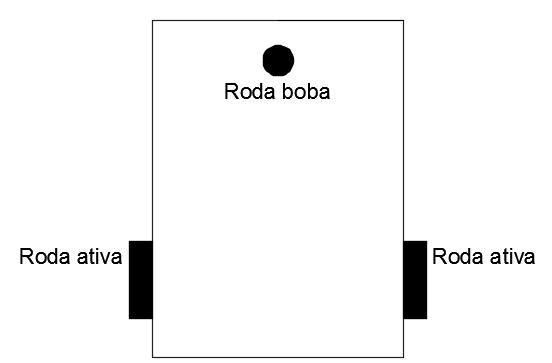
\includegraphics[width=0.75\textwidth]{figuras/robo bach.png}
    \caption{Esquema do chassi}
    \label{fig:chassi:robo}
\end{figure}
Para controle direcional utilizando os dois motores acoplados as rodas, foram criados modelos matemáticos que possibilitam calcular a rotação do robô tendo em vista a velocidade angular das rodas.

O algoritmo usado neste trabalho consiste em transformar o polígono descrito em uma matriz de números, onde 1's representam a área do polígono \ref{fig:matriz:poligono}. A escolha da melhor trajetória consiste em um problema de minimização de uma função-custo.
\begin{figure}[H]
    \centering
    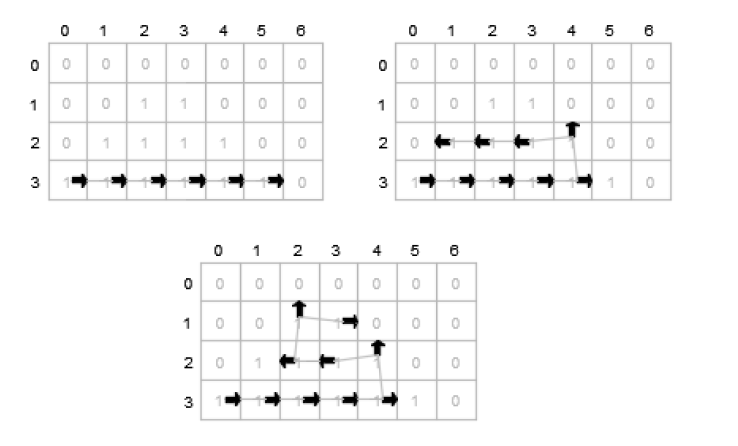
\includegraphics[width=0.75\textwidth]{figuras/matrizesPoligno.png}
    \caption{Esquema do chassi}
    \label{fig:matriz:poligono}
\end{figure}
\section{Autonomous Maneuvers of a Robotic Tractor for
Farming}

Com objetivo de diminuir a carga de trabalho dos trabalhadores rurais, a solução apresentada por \cite{Wang2016} aborda o controle de manobras para um trator de 4 rodas feito para trabalhar em plantações enfileiradas, bem como testes feitos em tipos diferentes de solo para avaliar a performance do mesmo.

O sistema foi construído utilizando um trator do modelo EG105 fabricado pela \textit{YANMAR} \ref{fig:yanmar:eg105} no Japão, além de cervos para controlar os ângulos de direção do mesmo. Para um posicionamento mais refinado do trator, utilizaram-se ainda um\textit{Real Time Kinematic Global Positioning System}(RTK-GPS) com a adição de dados de correção oriundas de uma rede chamada \texit{GPS Earth Observation Network}(GEONET)  disponível no Japão. 

\begin{figure}[H]
    \centering
    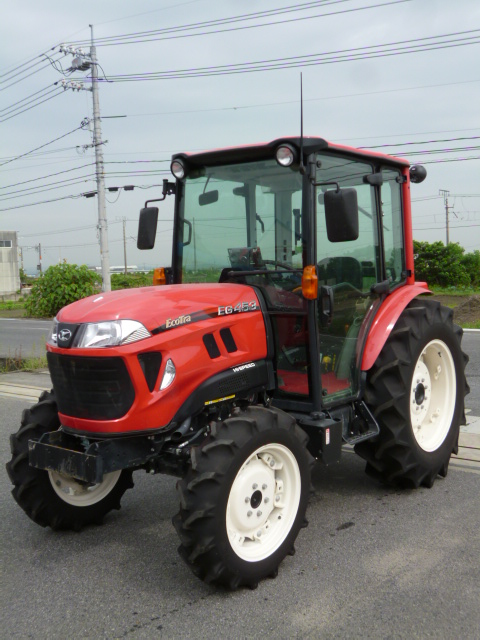
\includegraphics[width=0.55\textwidth]{figuras/EG105 yanmar.JPG}
    \caption{Yanmar EG105}
    \label{fig:yanmar:eg105}
\end{figure}

As manobras do trator foram programadas para imitar as manobras realizadas por operadores humanos, baseadas em arcos e círculos e seguimentos de reta. A direção desejada era determinada pela posição atual do trator e a posição de um ponto de navegação, os ângulos de curva são calculados baseados na diferença lateral e de direção do mesmo.

O sistema foi avaliado quanto a sua performance resultando em erros máximos de 10 centímetros entre a posição real do trator e a traçada pelos algoritmos, sendo que a diferença entre o vetor de direção real e o programado não passaram de 3º, provando que o mesmo pode operar de forma precisa sem necessidade de grandes mudanças de direção. Com esses resultados foi concluído que o robô trator pode operar autonomamente a 5km/h com erros aproximados de 6cm em relação a sua posição e 1.2º em relação ao vetor de direção.
\section{Path Planning Mobile Robot Using Waypoint
For Gas Level Mapping}

Dada a alta periculosidade envolvida na detecção de gases tóxicos, tanto de origem natural, bem como de origem da ação humana, cresceu a necessidade de automatizar os meios de detecção destes. Pensando nisso, foi desenvolvido um robô capaz de detectar gases tóxicos e se locomover seguindo pontos pré-estabelecidos, a fim de minimizar o possível contato humano com situações adversas à saúde.  Composto por quatro rodas e com sensores para detecção de gases, o robô foi montado sob um chassi de 4 rodas independentes como visto na \ref{fig:gas:chassi}. Para localização foram utilizados um GPS e compassos.
\begin{figure}[H]
    \centering
    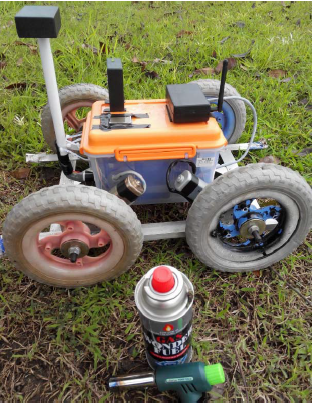
\includegraphics[width=0.55\textwidth]{figuras/chassi_robo_gas.png}
    \caption{Robô móvel utilizado}
    \label{fig:gas:chassi}
\end{figure}
A técnica utilizada para direcionar o robô foi baseada na premissa de que todas as rodas giram na mesma velocidade, logo, ao aumentar a velocidade de giro de uma delas, é mudada a direção do robô. Para direção, foram feitos cálculos baseados na posição atual do robô e a posição o próximo \textit{waypoint} e a diferença entre a direção do robô e a direção do waypoint. Depois disso, era calculada a distancia até o \textit{waypoint} usando a formula de Pitágoras. Durante a movimentação até o waypoint, dados são coletados tanto do GPS quanto do sensor de gases e enviados ao servidor através de um rádio.

Uma interface foi criada por \cite{Watiasih2017} onde pode-se ver os \textit{waypoints} e os pontos de presença de gases, além da leitura o sensor em tempo real. Nessa interface, apresentada na \ref{fig:gas:interface}, é possível também inserir os \textit{waypoints} a serem seguidos, tendo esses um número máximo de 100 para que não excedesse a capacidade de memória do robô.
\begin{figure}[H]
    \centering
    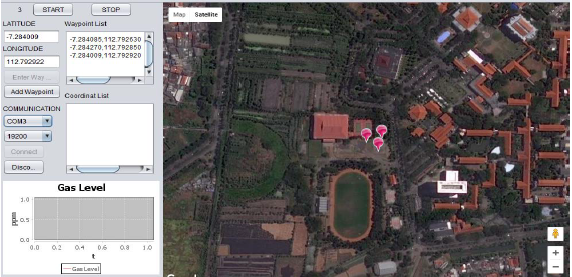
\includegraphics[width=0.7\textwidth]{figuras/interface_robo_gas.png}
    \caption{A interface conta com um mapa e caixas de textos para a inserção dos \textit{waypoints}}
    \label{fig:gas:interface}
\end{figure}
Testes levaram a um acerto de 95\% em relação a direção o robô e um erro de 3 metros em relação a posição real do \textit{waypoint}. Acredita-se que o número de satélites ao qual o GPS estiver travado interfira diretamente na precisão do mesmo.
\section{Scheduling and Control of Unmanned Ground Vehicles for Precision Farming: A Real-time Navigation Tool}

Este trabalho tem como objetivo a apresentação de um sistema para controle e agendamento  e veículos agrícolas autônomos com objetivo de executar agricultura de precisão de forma óptima. \cite{vlachos:2017} cara a hipótese elementar do trabalho dita que um campo e agricultura apresentam obstáculos, tanto aleatórios como estáticos, que um VAA deve detectar e recalcular seu caminho óptimo.  A grande contribuição deste trabalho vem da proposta de uma ferramenta de  \textit{software} em tempo real que reconheça o campo e guie o veiculo para suas tarefas enquanto proporcione um melhor uso dos recursos e, potencialmente, uma melhor colheita.

O sistema proposto visa navegar o VAA pelo campo para realizar tarefas de precisão, tais como fertilização, pulverização e plantio, para tal, ele é dividido em quatro partes: uma camada representando a paisagem; uma camada representando os objetos estáticos. Tais como arvores e pedras; uma camada representando os agentes de ação(VAA); uma camada representando as mensagens trocadas entre o nós do sistema e por fim uma camada que trata todas as informações , que prioriza e otimiza os caminhos do(s) VAA(s) no campo. Na questão do campo em si, são necessário dados sobre as fronteiras do campo, informações sobre potenciais obstáculos e a direção dos caminhos presentes no campo, bem como o \textit{layout} das plantações. São determinadas também as características quanto a tamanho do VAA afim o sistema conseguir calcular distancia seguras entre o mesmo e as plantações e/ou obstáculos. Com todas essas informações carregadas, bem como o \textit{feed-back} dos sensores presentes no VAA, o sistema é capaz de gerar um mapa e os caminhos a serem seguidos, como visto em \ref{fig:caminho-objetos-scheduling}, onde observa-se a disposição os objetos, bem como o caminho o VAA. 
\begin{figure}[H]
    \centering
    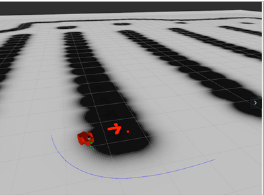
\includegraphics[width=0.7\textwidth]{figuras/caminho-objetos-scheduling.png}
    \caption{Representação gráfica dos dados disponíveis pelo sistema}
    \label{fig:caminho-objetos-scheduling}
\end{figure}
% falar sobre o LiDAR onde?
Os resultados comprovam a eficácia de tal abordagem, visto que com a adição dos sensores presentes no VAA, tais como o LiDAR que escaneia os arredores do VAA na busca por possíveis colisões, o mesmo consegue passar pela plantação com extrema precisão, possibilitando a utilização do mesmo em plantio em filas.
